%%
%% This is file `mcmthesis-demo.tex',
%% generated with the docstrip utility.
%%
%% The original source files were:
%%
%% mcmthesis.dtx  (with options: `demo')
%%
%% -----------------------------------
%%
%% This is a generated file.
%%
%% Copyright (C)
%%       2010 -- 2015 by Zhaoli Wang
%%       2014 -- 2019 by Liam Huang
%%       2019 -- present by latexstudio.net
%%
%% This work may be distributed and/or modified under the
%% conditions of the LaTeX Project Public License, either version 1.3
%% of this license or (at your option) any later version.
%% The latest version of this license is in
%%   http://www.latex-project.org/lppl.txt
%% and version 1.3 or later is part of all distributions of LaTeX
%% version 2005/12/01 or later.
%%
%% This work has the LPPL maintenance status `maintained'.
%%
%% The Current Maintainer of this work is Liam Huang.
%%
%%
%% This is file `mcmthesis-demo.tex',
%% generated with the docstrip utility.
%%
%% The original source files were:
%%
%% mcmthesis.dtx  (with options: `demo')
%%
%% -----------------------------------
%%
%% This is a generated file.
%%
%% Copyright (C)
%%       2010 -- 2015 by Zhaoli Wang
%%       2014 -- 2019 by Liam Huang
%%       2019 -- present by latexstudio.net
%%
%% This work may be distributed and/or modified under the
%% conditions of the LaTeX Project Public License, either version 1.3
%% of this license or (at your option) any later version.
%% The latest version of this license is in
%%   http://www.latex-project.org/lppl.txt
%% and version 1.3 or later is part of all distributions of LaTeX
%% version 2005/12/01 or later.
%%
%% This work has the LPPL maintenance status `maintained'.
%%
%% The Current Maintainer of this work is Liam Huang.
%%
\documentclass{mcmthesis}
\mcmsetup{CTeX = true,   % 使用 CTeX 套装时,设置为 true
        tcn = 2013573, problem = E,
        sheet = true, titleinsheet = true, keywordsinsheet = true,
        titlepage = false, abstract = true}
\usepackage{newtxtext}%\usepackage{palatino}
\usepackage{lipsum}
\usepackage{caption}
\usepackage{subfigure}
\usepackage{float}
\usepackage{verbatim}
\title{塑料Global Plastic Waste Model based on Linear Programming and Support Vector Regression}
\author{Team 2013573}
\date{\today}
\begin{document}
\begin{abstract}

Plastic waste (PW) has been one of intractable environmental dilemma for modern humankind. In order to mitigate this tough problem, we combine production of plastics and management of plastic waste to establish a model, which can evaluate the impacts of plastic waste and find out an achievable minimal level of plastic production that can be reduced with a time line.  

Firstly, we develop a plastic waste estimate model based on Product Life Cycle (PLC) theory to calculate the maximal levels of single-use or disposable plastic product waste within the environmental capacity in a certain region or country. Then we independently explore the four possible ends of PW and formulate their impacts on environment by several functions. We use linear programming that includes one particular objective function and four constraints. As a result, we can output the maximal amount of plastic products by analyzing the input digits of any region. 

Secondly, to find out to what extent plastic waste can be minimized, we established an model called HSVR which combines happiness-index analysis and SVR method. By analyzing the characteristics of different regions and people’s living standards, we find out the relationship between the amount of plastics produced and people’s happiness index. Based on this, we can analyze how much plastic production we can reduce without significantly reducing happiness.

Thirdly, we follow the previous happiness index to assess how much human life is changed, and apply the Environmental Assessment of Solid Waste Systems and Technologies (EASEWASTE) model to evaluating how the the environment is affected by plastic reduction. Moreover, we take computable general equilibrium (CGE) model to quantify the effects of the target plastic production. Then we normalized the outputs and into non-dimensional indices, and calculate the weight for each indicator above by the analytic hierarchy process (AHP). The total impact for achieving the confined level is a linear combination of the three indices. 

Furthermore, reduction of plastic production will impact countries unequally because of their different development level. We use dual programming to fine the dual model of the linear programming based model we established first. Then shadow prices of every factor formulated by constraints can be calculated, which indicate the significance of each factors. Then we divided them into environmental and governmental factors. Sensitivity analysis is be used to identify which factors that is most sensitive to a particular country, and the equitable reduction of plastic of the country depends on the categories that its sensitive factors belong to. 

Finally, we analyze how to approach the minimum level following the time line by an achievable way. Many unexpected circumstance would definitely appear so we empirically choose most significant possibilities that may delay or accelerate the achievement process. The ultimate result are specified into a memo which will be provided for ICM.

\begin{keywords}
Plastic waste; LCA; SVR; EASEWASTE; AHP
\end{keywords}
\end{abstract}
\maketitle
%% Generate the Table of Contents, if it's needed.
\thispagestyle{empty}
\tableofcontents
\thispagestyle{empty}
\newpage
%\setcounter{page}{1}
%%
%% Generate the Memorandum, if it's needed.
\memoto{ICM officials}
\memofrom{Team 2013573}
\memosubject{Global Plastic Waste Issue}
\memodate{\today}
%\logo{\LARGE I'm pretending to be a LOGO!}
\begin{memo}[Memorandum]

It is a great honor for us to be hired to address this increasingly severe situation crisis. Current global plastic waste has exceeded the environmental tolerance level, therefore an achievable level of reducing plastic waste is badly needed. Considering the mutual influence between plastic industry and human community, we have managed to find out an appropriate global target minimum of single-use plastic waste and the timeline to meet it. 

We are pleased to tell you that we make it to estimate an appripriate target for a specific country. In Section4, the impact of plastic usage on human licing standards is explored by SVR algorithm. And based on the thought of not affecting much of human living standards, training results of different SVR kernel functions are utilized to predict minimum plastic usage in a particular area. 

As for the global target mimimum achievable levels of single-use or disposable plastic product waste that we both concern most,  we divided the world into 10 typical countries according to their plastic consumption amount,  and for each category of countries the target for minimum plastic use is calculated. Then add up those predicted outcomes and a global target minimum achievable target is obtained. As we demostrate in our paper, the total minimal plastic consumption obtained is about 6.6 hundred million tons.

Every target needs a schedule to  realize, no mention to this grand plane to make the global plastic production and usage reach the defined level. Hence we need design a feasible timeline to achieve this level. However, according to our sensitivity analysis results, countries have various sensitivity to every single factor. It seems unrealistic to set the same timeline for all countries because they are in different industry structures.  So the better way is to consider several timelines separately for disparate countries. 


The majority of developed country has developed mature services. Although they use a lot of plastics, their plastic waste have been managed well due to their advanced recovery technologies. For them, reducing plastic means higher quality and efficiency of management. This is not a difficult task, but it requires a lot of perseverance and determination. However, manufacturing takes a prior part of domestic economy in most developing country and reducing the production of plastic is likely to threaten economy growth. For developing countries, reducing the use of plastic is a pain, because it means slowing development. In order not to deprive of the right of development of poor population, we suggest a loose timetable for medium-income and low-income countries to optimize their industrial structure and reduce plastic waste.

Given all above we discussed, we decide to propose the timelime as follow:

By 2035, developed countries will first achieve reductions to established targets, and will begin to study how to further reduce the use of plastic. 
By 2050, all countries around the world will reach a lower level of plastic use. 

The main consideration of this timeline is that the amount of plastic used in developed countries is much larger than that in developing countries, but they pay less to reduce it than in developing countries, as is presented before. But this issue cannot be generalized. For example, for the case we studied in China, the biggest problem is actually improper management. However, environmental and industrial factors cannot be ignored. The best way is to use our model to study all regions of the world as closely as possible to get an exact answer. This may be a laborious task, but it is definitely worth it.

There is a long way to go to achieve this goal between now and the future.  So we list some circumstances that may affect the achievement of the target:

As for technology, if relevant research about plastic waste managing make remarkable progress and the findings are quickly implemented by environmental sector, the process of plastic reduction will be accelerated. 

Besides, taking economic growth into account, it is likely that the government loosen regulations of plastic management in a recession to guarantee the economic growth. Take Bolsonaro administration for example, local government usually attach less importance to environmental issues.

Wish the given advice above would contribute to your work!

\thispagestyle{empty}

\end{memo}

%%
\setcounter{page}{1}
\section{Introduction}
\subsection{Background}

The plastic industry can date back to1950s. Over the past 60 years, the production of plastic has grown rapidly, which has surpassed most other artificial materials\cite{Geyer}. While people then did not realize the potential negative influence of plastic usage to ecosystem, plastic waste gradually accumulated in the environment because of it’s non-biodegradable trait. Some scholar believe that plastic bags and Styrofoam containers can take up to 1,000 years to decompose\cite{Giacovelli}. 6,300Mt plastic waste has been generated in 2015, while only 9\% of which had been recycled and reused. 12\% of them were incinerated and the percentage of plastics that discarded in landfills or natural environment was up to 79\%\cite{Geyer}. Plastics in nature especially in the ocean will cause a series of ecological problems. Apart form the chemical affects to organisms, plastic ingestion and entanglement are also threatening the diversity of species\cite{LI}. It is easy to imagine that if no measure is taken, human will facing severe degradation and pollution caused by enormous plastic waste.

Besides, the management of the plastic waste is one of the hardest issue on integrated municipal solid waste. There are many researches that focus on the plastic recovery routes based on the life cycle assessment approach (LCA) \cite{Rigamonti}, and a few methods to assess the impact of solid waste system and technologies, which aim at develop more effective ways to migrate the plastic waste problem\cite{Kirkeby}.

However, it seems that there are few researchers that explored the valuation model of estimating the maximal use of plastics nor utility policy to reduce the usage of plastics remarkably. That indicates there is still room for further explanation in this area. 

%The management of the plastic waste is one of the most controversial topic in the discussion on integrated municipal solid waste area.

\subsection{Problem statement}

Living in the age that are characterized by a series of  troublesome environmental problems, such as global warming, desertification, pollution of water and poor air quality. Our team is hired to estimate the maximal permitted amount of plastic products, migrate the plastic production and reduce plastic waste. In another word, we need to answer the following questions:

\begin{enumerate}
	\item What is the maximal level of single-use or disposable plastic products without further pollution?
	\item What extent can plastic waste be reduced to?
	\item What is the minimal achievable level of global single-use or disposable plastic products and what are the impact on certain facets of reaching this level?
	\item How to solve the equity problem about plastic waste that arise from global crisis?
	\item How to build a timeline to approuch our target level we set before and describe our exploration to ICM?
\end{enumerate}

%\subsection{Our work}
%
%Our work can be summarized as follows:
%
%\begin{itemize}
%	\item To get the maximal level of single-use or disposable plastic products, we build PWEM on the basis of LCA, and applied some logical abstractions, physical derivations, and mathematical methods to accomplished the linear programming process, then out put the estimated maximal level of plastic products. 
%	\item We create our HSVR model to define the miximal level with least negative effects on people’s  living standards, based on the fact that people often do not agree to pay too much for environmental protection.
%	\item Using our moedl, we set an achievable target level of plastic usage and apply quite a few known methods to quantify and combine the given factors for assessing the total influence of achieving our goal. 
%	\item We developed our model to measure the influence of various factors to provide realistic solutions for the mentioned euity issue.
%\end{itemize}

%For task 5, TSM is established for predicting the possible timeline and discuss possible relevant circumstances, then write a specific memo for ICM.

\section{Model Analysis}
\subsection{Analysis of task 1}

\section{Assumptions and justifications}

To simplify the problem, we strive for the following assumptions:

\begin{itemize}
	
	\item \textbf{The mass of annual plastic production equals to that of the annual plastic waste.} On the one hand, every pound of plastic produced will turn into waste. On the other hand, the lifeline of most sorts of plastic is under 20 so that given situation will not change acutely\cite{Geyer}.
	
	\item \textbf{Throughout the life cycle of plastic, the impact of plastic on environment in use phase is negligible.} Main environment issues that are related to plastic merely when it is produced or managed\cite{book}.
	
	\item \textbf{Aiming to make plastic waste safely be mitigated, any waste should not be landfilled.} While it is extremely hard for plastic to biodegrate in solid, landfills are in great shortage.\cite{book}.
	
	\item \textbf{All the plastic waste produced will be managed.} In the long run, the NET plastic waste discarded in natural environment will approach zero by governments and NGOs’ efforts.
	
	\item \textbf{The proper quantity of pollutant emission of plastic waste should depend on the contribution of plastic industry to the gross domestic products.} The pollutant emission of plastic waste is just an ordinary part of the total emission, so the responsibility of environmental protection it takes should also be the proportional part, which is roughly estimated by the percentage of GDP that plastic industry contributes.
	
	\item \textbf{All the plastic waste is mechanically sorted from plastic waste prior to incineration.} In fact, waste incineration plants are generally very formal and will complete the sorting work. Otherwise, they will be banned soon.
	
	\item \textbf{The material recycling facilities(MRFs) that sort and upgrade the received waste stream is the only way to recycled sorted PW.} There is no other mature processing method, and this method is used almost everywhere.
	
\end{itemize}

\section{Parameter Table}

Important symbols that in this article are listed in Table \ref{notation}.
\begin{table}[H] 
	\caption{Notations} 
	\center
	\begin{tabular}{cp{0.7\columnwidth}}
		\toprule 
		Symbols &Definition  \\ 
		\midrule 
		$s_i $& Annual certain plastic production.  \\ 
		$N_i$ & The number of $CO2$ generated by the combustion of 1 molecule specific plastic unit. \\ 
		$EA$ & Emission to air. \\ 
		$EW$ & Emission to water.\\
		$EC$ & Emission of $CO_2$.\\
		$TEA$ & Total emission to air.\\
		$TEW$ & Total emission to water.\\
		$TEC$ & Total emission of $CO_2$.\\
		$CEA$ & Compensatory emission to air of recovery process.\\
		$CEW$ & Compensatory emission to water of recovery process.\\
		$SM$ & Plastic waste into marine.\\
		$M$ & The quantity of annual management of marine plastic.\\
		$V_air$ & Total available air of a specific country/region.\\
		$V_water$ & Total available water of a specific country/region.\\
		$\sigma$ & Proportion of incinerated plastic waste.\\
		$\mu$ & Compensate.\\
		$\theta$ & The percentage of GDP plastic industry contributes, quantified by coefficient.\\
		$\iota$ & Tossil fuel consumption percentage. Generally, $\iota$ equals 4\%.\\
		$k$ & Proportional coefficient of carbon emission per unit of
energy consumption\\
		\bottomrule 
		\label{notation}
	\end{tabular} 
\end{table}

\section{Model for maximal plastic waste estimation based on Linear programming}
\label{lp}

%We noticed that this puzzle is a maximization problem with several limiting conditions. So linear programming(LP) must be the best way to approach the answer we want.

Maximal plastic waste is a problem related to plastic production, using, and recycling. Based on LCA, we analyzed all the pollution generated in the life cycle of plastics, and then reduced this problem into a linear programming model. Finally, we use the simplex method to solve based on an example.

\subsection{Theories related to our model}

In this section, we will introduce theories that are closely related to our model.

%%PLC theory tell us the specific stage of plastic life will impact environment, while LCA theory provide us a tool to quntify impacts of recyclement. LP and simplex algorithm(SA) are mathematical methods, and by former we establish our objective functions and constraints while by the latter  we get the optimal solution for LP.

\subsubsection{PLC theory}

To guarantee that the maximal usage or producing of plastics will not damage the environment further, we identify the parts of plastics’ life cycle that might cause damage to the environment, as is shown in figure \ref{fig4}. Consider a revised product life cycle (PLC) theory: as every product has its life cycle from R\&D(\textbf{esearch and development}) to launching on market to decline and exit the market as an end, plastics also cycle from products to waste. For plastic products from various source, their producing processed may affect the environment as well as their managing courses. The model expand based on the plastic life cycle theory. 

\begin{figure}[!htb] %H为当前位置,!htb为忽略美学标准,htbp为浮动图形
	\centering %图片居中
	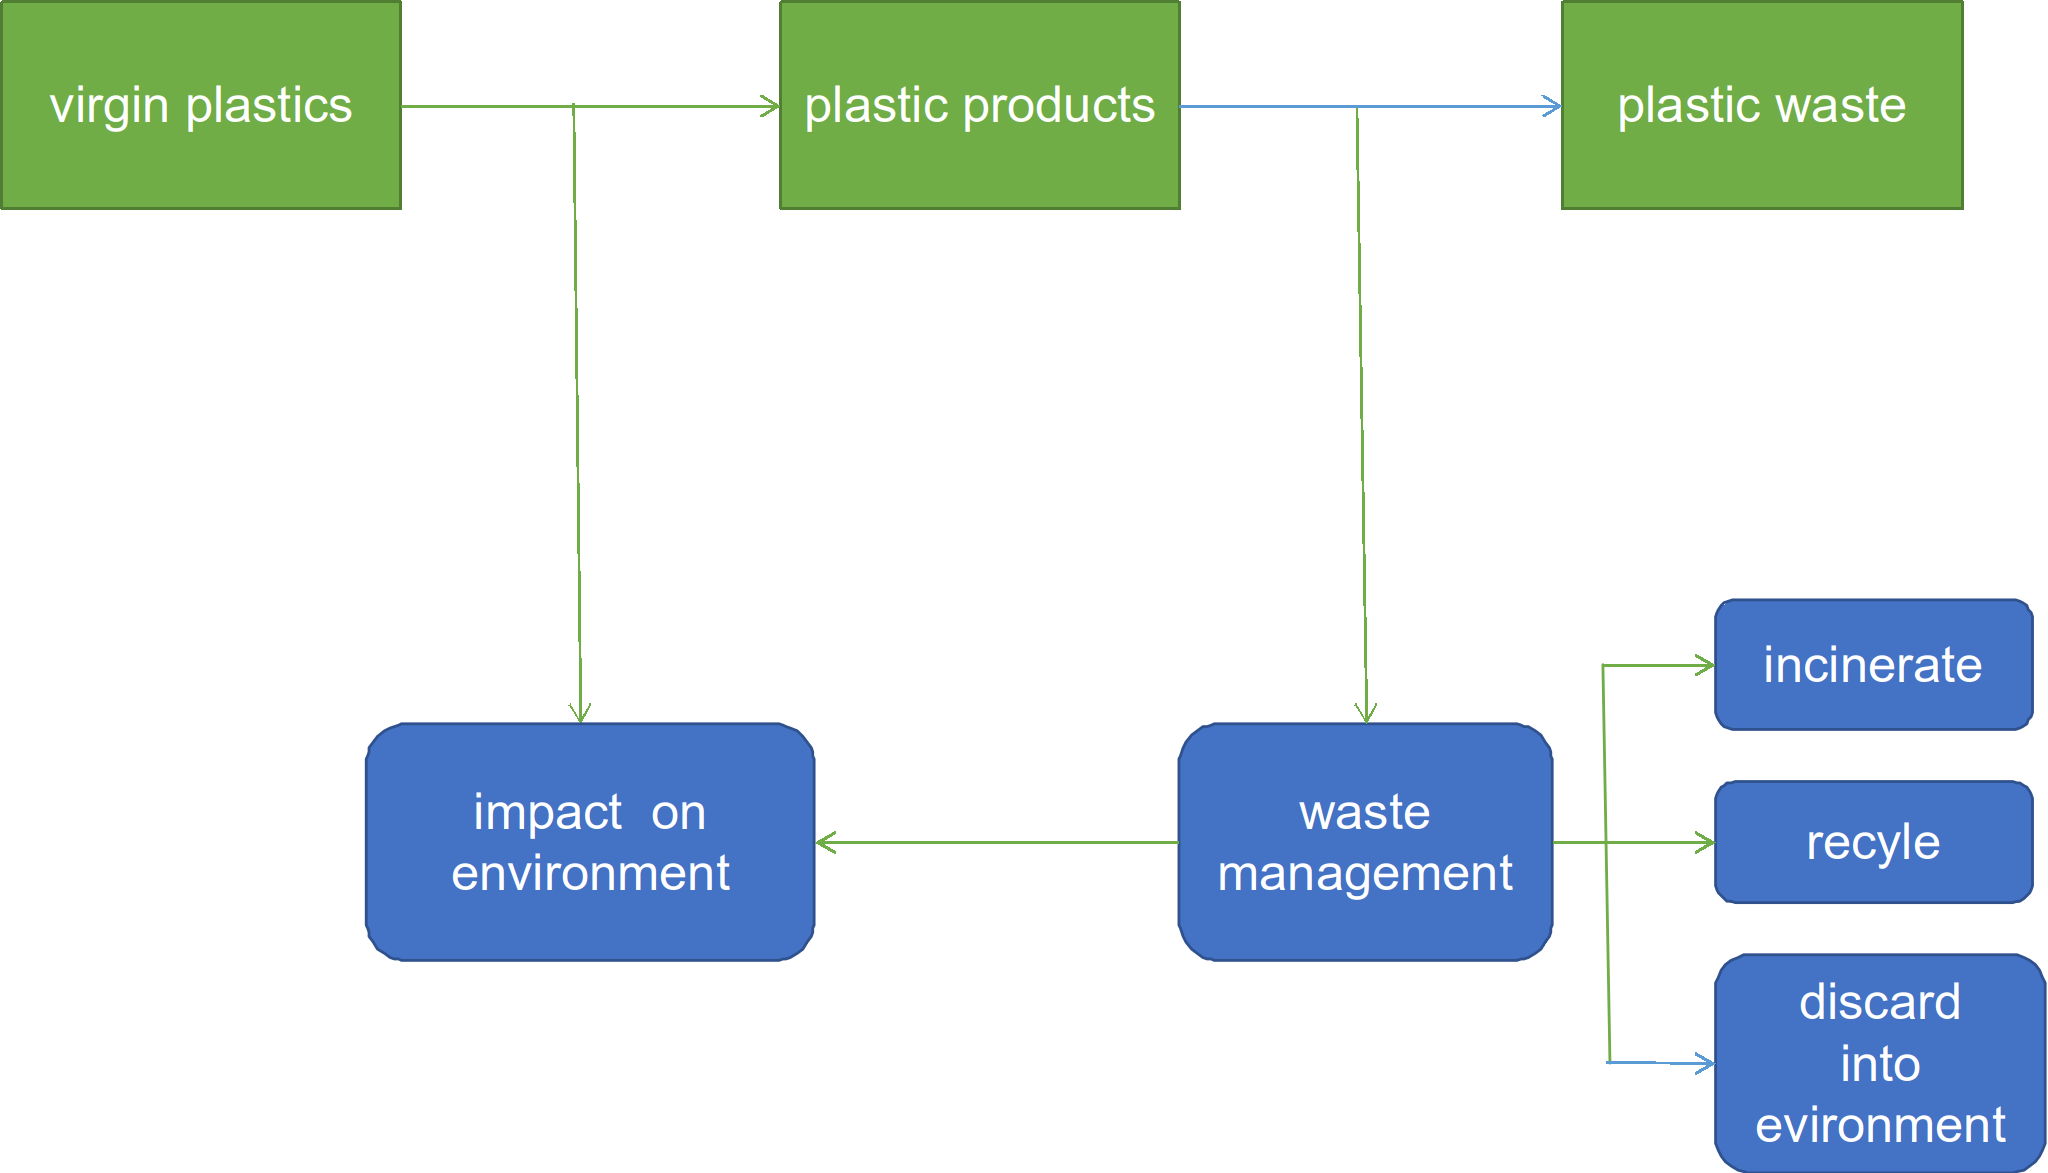
\includegraphics[width=0.7\textwidth]{figures/PCL.png} %插入图片,[]中设置图片大小,{}中是图片文件名
	\caption{The parts of plastics’ life cycle that might cause damage to the environment.} %最终文档中希望显示的图片标题
	\label{fig4} %用于文内引用的标签
	
\end{figure}

\subsubsection{Linear programming}

Linear programming\cite{Hillier} (LP) is a tool for solving optimization problems for which we do following:

\begin{enumerate}
	\item We attempt to maximize (or minimize) a linear function of the decision variables which is called the objective function. 
	\item The values of the decision variables must satisfy a set of constraints. Each constraint must be a linear equation or linear inequality.
	\item A sign restriction is associated with each variable. For any variable $x_i$, the sign restriction specifies that $x_i$ must be either nonnegative ($xi \ge 0$) or unrestricted in sign.
\end{enumerate}

So we try to set our objective function as the permitted maximal amount of plastic and abstract the most limited conditions into constraints.

%\subsection{Notations}
%
%The notations used are shown in table \ref{notation}.



\subsection{Qualify the impact on the environment}

We analyzed the pollution caused by each stage of the plastic's entire life cycle.

\subsubsection{Producing process}

According to the first assumption, we consider the annual production and waste as the same variable $S$. And naturally it is divided into various sorts of plastic.

\begin{equation}
S = \sum_i{s_i}
\label{S}
\end{equation}

Note that, $i$ rrepresents a sort of plastic and $s_i$ is the annual production of this sort of plastic. All sorts of plastic taken into account are PVC, PE, PP, PS, PET, PUR and PC\cite{book}.

To quantify to what extent plastic waste impact the environment in its life cycle, we use Emissions air($EA$) and Emissions water ($EW$) to measure emissions, whose units are Units of Polluted Water ($UPW$/ton) and Unit of Polluted Air with the production of a ton of plastic($UPA$/ton). $UPW$ is the number of cubic meters of water polluted up to the European drinking water standard by the production of 1 tonne of the material. $UPA$ is a similar measure for air and gives the cubic meters of air needed to dilute the emissions to the European maximum acceptable concentration (MAC)\cite{book}. Then the Emissions of water and air can be formulated below:

\begin{equation}
TEA^{\alpha} = \sum_i{s_i}\times EA_i^\alpha
\label{EA}
\end{equation}

\begin{equation}
TEW^{\alpha} = \sum_i{s_i}\times EW_i^\alpha
\label{EW}
\end{equation}

Given the energy consumption per unit of plastic production, we set energy consumption of specific plastic production as $E_i$ and the proportional coefficient of carbon emission per unit of energy consumption as $k$, total emission of CO2 can be calculated as: 

\begin{equation}
TEC^\alpha = k\sum_i{s_i}\times E_i^\alpha
\label{EC}
\end{equation}

%Additionally, in the process of incineration, we take the Emission of greenhouse gases CO2($EC$) into account.

%\begin{equation}
%%TEC = \frac{\sigma}{1+\sigma}\sum_i{s_i}\times N_i
%\label{EC}
%\end{equation}

%%\begin{equation}
%%TEC = \sum_i{s_i}\times E_i^\alpha
%%\label{EC}
%%\end{equation}

%Note that the superscript $\alpha$ means the process of plastic production. Similarly, replace $\alpha$ with $\beta$ means the process of plastic waste management.

\subsubsection{Managing process}

When it comes to plastic waste management, there are three possible fates for managed plastic waste: being recycled, being incinerated and being discarded(be landfilled or be discarded in natural environment). According to the third and fourth assumption, we assume there are only two managing method: incinerating or recycling.

%When it comes to plastic waste management, there are three possible fates for managed plastic waste: be recycled, be incinerated or be discarded(be landfilled or be discarded in natural environment). According to the third and fourth assumption, we don’t take the part of waste discarded into account. And the proportion of the recycled part and the incinerated part(symbolized by ) is given by scenario P4 in paper\cite{Rigamonti}. Then the environmental impact of plastic waste management can be calculated:

For the proportion of recycled PW, they are recycled by The material recycling facilities(MRFs). The mechanical separation removes polyethylene terephthalate (PET) and high density polyethylene(HDPE) bottles at high efficiency, which are sent to recycling, and other minor high calorific fluxes sent to energy recovery in cement kilns\cite{Rigamonti}. After that we could get certain recovery rate, we set this rate as $1 - \sigma$, the proportion of incinerated part is $\sigma$.

Firstly, we apply a classical environmental assessment method: life cycle assessment (LCA), to evaluate the environmental issues associated with solid wast with solid waste management\cite{Kirkeby}.

\begin{comment}

The following impact categories have been assessed:

\begin{itemize}
	\item Global warming potential (GWP) 
	\item Photochemical ozone creation potential (POCP)
	\item Eutrophication potential (EP)
	\item Acidification potential (AP)
	\item Human toxicity potentials (HTP)
	\item Ozone layer depletion potential (OLDP)
	\item Abiotic depletion potential\cite{Shonfield} (ADP)
\end{itemize}

\end{comment}

Secondly, we simplify and abstract the many categories of LCA into three categories based on data availability and computational matching: EA, EW and EC.

Furthermore, because the recycling technology(MRFs) saves this part of PW from incineration and put recycled products into market again, while the harmful emissions from recycling are often less than the emissions from incinerating this part of the plastic\cite{Shonfield}. There are digital supports that reveal the positive influence about of recovery, as is shown in figure \ref{fig6} and figure \ref{fig7}. So we calculate this different value as compensatory emissions.

\begin{figure}[!htb] %H为当前位置,!htb为忽略美学标准,htbp为浮动图形
	\centering %图片居中
	\includegraphics[width=0.7\textwidth]{figures/PCA1.png} %插入图片,[]中设置图片大小,{}中是图片文件名
	\caption{Net eutrophication potential.} %最终文档中希望显示的图片标题
	\label{fig6} %用于文内引用的标签
	
\end{figure}

\begin{figure}[!htb] %H为当前位置,!htb为忽略美学标准,htbp为浮动图形
	\centering %图片居中
	\includegraphics[width=0.7\textwidth]{figures/PCA2.png} %插入图片,[]中设置图片大小,{}中是图片文件名
	\caption{Net global warming potential.} %最终文档中希望显示的图片标题
	\label{fig7} %用于文内引用的标签
	
\end{figure}

\begin{comment}

\begin{figure}[htbp]
	\centering    %居中
	
	\subfigure[name of the subfigure] %第一张子图
	{
		\begin{minipage}[t]{0.5\linewidth}
			\centering          %子图居中
			\includegraphics[scale=0.7]{PCA1.png}   %以pic.jpg的0.5倍大小输出
		\end{minipage}
	}
	
	\subfigure[name of the subfigure] %第二张子图
	{
		\begin{minipage}[t]{0.5\linewidth}
			\centering      %子图居中
			\includegraphics[scale=0.7]{PCA2.png}   %以pic.jpg的0.5倍大小输出
		\end{minipage}
	}
	
	\caption{name of the figure} %  %大图名称
	\label{fig5}  %图片引用标记
\end{figure}

\end{comment}

Then the environmental impact of plastic waste management can be calculated:

\begin{equation}
TEA^\beta = \sigma\sum_i{s_i}\times EA_i^\beta - (1 - \sigma)\sum_i{s_i}\times CEA_i^\beta
\label{EAB}
\end{equation}

\begin{equation}
TEW^\beta = \sigma\sum_i{s_i}\times EW_i^\beta - (1 - \sigma)\sum_i{s_i}\times CEW_i^\beta
\label{EWB}
\end{equation}

%where $N_i$ is the number of $CO_2$ generated by the combustion of 1 molecule specific plastic unit. The superscript $\beta$ is omitted because only the incineration process emit $CO_2$.

Apart from above analysis, although we assume that all the plastic waste discarded in natural environment will be managed, too much discarded plastic waste (even if temporarily) will notably do harm to marine ecosystem\cite{LI}. Thus it’s necessary to estimate the mass of plastic waste(symbolized by $SM$) inputs from land into the ocean, given specific total plastic waste.

\begin{equation}
SM = \varsigma\sum_i{s_i}
\label{SM}
\end{equation}

%$\varsigma$ is the empirical coefficient of $SM$ and total mass of plastic waste, calculated by former statistics.

For the plastic waste that has been incinerated, in the process of incineration, we take the emission of greenhouse gases $CO_2$ (EC) to represent it’s contributions to global warming:

\begin{equation}
TEC^\beta = \sigma\sum_{i}s_i\times N_i - \mu(1 - \sigma)\sum_is_i
\end{equation}

\subsection{Constraints given by environmental carrying capacity}

Firstly, according to the fifth assumption, the pollutant emission constraints are roughly estimated by the percentage of GDP plastic industry contributes, quantified by coefficient $\theta$.

\begin{equation}
TEA^\alpha + TEA^\beta \le \theta V_{air}
\label{air}
\end{equation}

\begin{equation}
TEW^\alpha + TEW^\beta \le \theta V_{water}
\label{water}
\end{equation}

%$V_{air}$ and $V_{water}$ is the total available air/water of a specific country/region.

Secondly, when it comes to greenhouse gas $CO_2$, it’s more propriate to use its fossil fuel consumption percentage to set the restraint because the fossil fuel combustion is the principal factor of the global warming, rather than natural carbon cycles\cite{book}.

\begin{equation}
TEC^\alpha + TEC^\beta \le \iota V_{CO_2}
\label{ECO}
\end{equation}

%where $V_{CO_2}$ is the promised maximal $CO_2$ emissions of specific country or region and $\iota$ is fossil fuel consumption percentage. Generally, $\iota$ equals 4\%.

Last but not least, considering current quantity of plastic discarded in the ocean don’t exert severe impact on marine ecosystem, we regard zero net input into the sea an acceptable circumstance for marine environment, i.e. annual plastic waste input can’t beyond the quantity of annual management of marine plastic(symbolized by $M$).

\begin{equation}
SM \le M
\end{equation}

%Finally, we can synthesize the formulas above, solve the constrained optimization problem and obtain the maximum levels of plastic product waste.

\subsection{Model paradigm}

In the end, our model can be written as follows:

Objective functions:

\begin{equation}
S = \sum_i{s_i}
\label{z}
\end{equation}

subject to:

\begin{equation}
\label{eq6}
\left\{
\begin{aligned}
TEA^\alpha + TEA^\beta \le \theta V_{air}\\
TEW^\alpha + TEW^\beta \le \theta V_{water}\\
TEC^\alpha + TEC^\beta \le \iota V_{CO_2}\\
SM \le M
\end{aligned}
\right.
\end{equation}

\subsection{Analysis of China using our model}

In this section, we will combine the data from China to further introduce the model.

China is a developing country which emission largest amount of PW to marine, which may be sensitive to change of plastic amount. As shown in figure \ref{fig09}, China has the most and most developed plastic industry in the world. We apply our model to the practical examples of China. Table \ref{type} lists seven disposable plastics mainly used in China. We consider them as model variables $s_i$.

\begin{figure}[!htb] %H为当前位置,!htb为忽略美学标准,htbp为浮动图形
	\centering %图片居中
	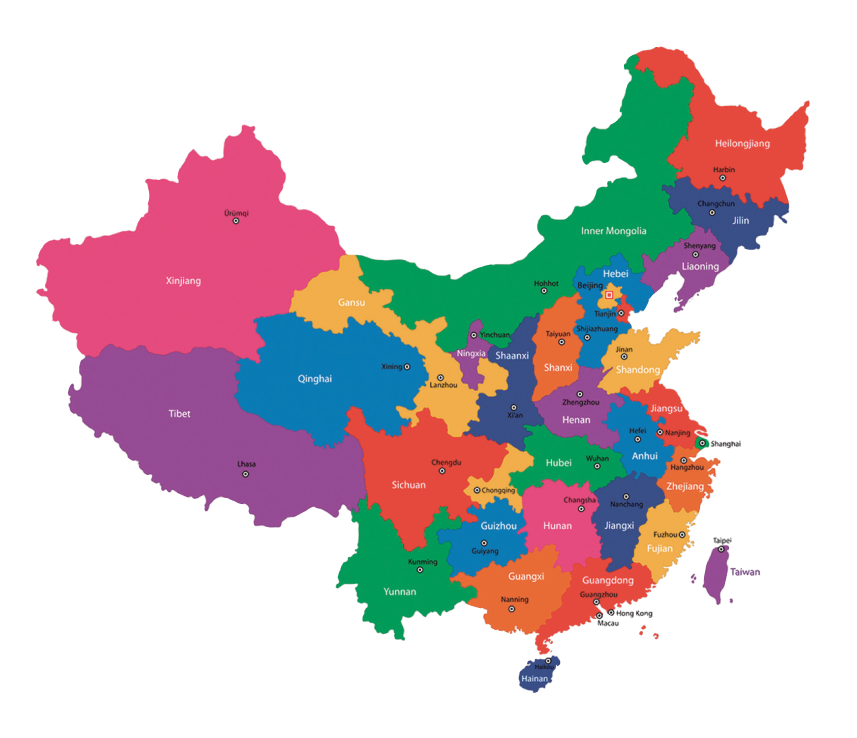
\includegraphics[width=0.7\textwidth]{figures/Map.png} %插入图片,[]中设置图片大小,{}中是图片文件名
	\caption{China's developed plastic industry.} %最终文档中希望显示的图片标题
	\label{fig09} %用于文内引用的标签
	
\end{figure}

\begin{table}[]
	\center
	\caption{The main types of disposable plastics used in China}
	\label{type}
	\begin{tabular}{|c|c|}
		\hline
		\textbf{Variable} & \textbf{Plastic types} \\ \hline
		s1                & PVC                    \\ \hline
		s2                & PE                     \\ \hline
		s3                & PP                     \\ \hline
		s4                & PS                     \\ \hline
		s5                & PET                    \\ \hline
		s6                & PUR                    \\ \hline
		s7                & PC                     \\ \hline
	\end{tabular}
\end{table}

We used data from the National Bureau of Statistics of China\cite{Country} and obtained parameters closely related to the model. Specific information can be consulted in the appendix.

Note that for practical reasons, we set some settings for the model, where the compensite emission to water and air of recycling process should be deemed as zero for the following considerations:

\begin{enumerate}
	\item The proportion of recycled PW is relatively small in realistic practices. 
	\item Most regions of China are not developed enough to have the advanced technology of MRFs to manage PW.
	\item Chinese PW sorting and managing system are not perfect.
\end{enumerate}

Finally, the linear programming model based on Chinese data is as Eq.\ref{sc} and Eq.\ref{cc}:

\begin{equation}
	S = s_1 + s_2 + s_3 + s_4 + s_5 + s_6 + s_7
	\label{sc}
\end{equation}

\begin{equation}
\label{cc}
\left\{
\begin{aligned}
700s_1+265s_2+325s_3+255s_4+180s_5+0s_6+180s_7\le 2.88\times 10^{11}\\
3000s_1+1650s_2+3685s_3+6355s_4+8000s_5+0s_6+5050s_7\le7.89696\times 10^{10}\\
1.99s_1+4.42s_2+4.43s_3+4.77s_4+3.23s_5+0.49s_6+1.96s_7)\le 8.062\times 10^{11}\\
0.41\times(s_1+s_2+s_3+s_4+s_5+s_6+s_7)\le 4.85\times 10^5
\end{aligned}
\right.
\end{equation}

%Given the compensatory emission of recycling process is a relatively vague variable for three reasons:

%Given all above realistic situations, the compensite emission to water and air of recycling process should be deemed as zero, so is the compensite coefficient of $CO_2$.

We solved this problem by using the simplex method through MATLAB, and obtained the largest amount of plastic that China can bear in one year. The results show that China can bear 1.18 million tons of plastic a year. When the optimal solution is obtained, the production volume of various plastics is shown in table\ref{aos}.

\begin{table}[]
	\center
	\caption{The amount of various plastics in the optimal solution}
	\label{aos}
	\begin{tabular}{|c|c|}
		\hline
		\textbf{Plastic types} & Amount of plastic(t) \\ \hline
		PVC                    & 210428.703365915     \\ \hline
		PE                     & 107339.181740866     \\ \hline
		PP                     & 174475.173021043     \\ \hline
		PS                     & 150364.822097472     \\ \hline
		PET                    & 233445.923823156     \\ \hline
		PUR                    & 42560.4917899467     \\ \hline
		PC                     & 264312.533429888     \\ \hline
	\end{tabular}
\end{table}

We will continue to analyze this case later to explore the impact of different constraints.

\section{Plastic waste reduced}

\label{p2}

At present, the global use of plastics has exceeded the upper limit of environmental tolerance, which poses a huge threat to the ecological environment. Considering the huge differences in the existence of countries around the world, we must consider each region separately. In section \ref{p2}, we propose a model of Happiness based on SVR\cite{Smola}, which we call HSVR. Using HSVR, we will explore the impact of the use of plastic on human living standards in a region, and try to reduce the amount of plastic used as much as possible without affecting much of human living standards.

Our method can be summarized as follows: the use of plastic is essential, and reducing the use of plastic will inevitably affect the living standards of local people. By analyzing the characteristics of different regions (especially the amount of plastics consumed) and the people's living standards, we find out the relationship between the amount of plastics consumed and the people's happiness index. Based on this, we can analyze how much plastic consumption we can reduce without significantly reducing the happiness index.

The following of this section will first briefly introduce the method we use, and then obtain a specific regression model based on the Global Happiness Report\cite{World} and plastic consumption in each region\cite{Plastic}.

\subsection{SVR algorithm}

Support vector regression(SVR) is an application of SVM (support vector machine) to regression problems. Support vector machines construct a hyperplane or a series of hyperplanes in a high-dimensional or infinite-dimensional space, which can be used for classification, regression, or other tasks. Intuitively, using a hyperplane to achieve a good segmentation can make the closest training data points have the largest separation distance in any category. This is because usually a larger margin can have a lower generalization error of classifier\cite{SVRs}.

Given training vectors $x_i \in R^p, i = 1, \cdots, n$, and a vector $y \in R^n$. $\varepsilon-SVR$ solves the following primal problem:

\begin{equation}
\min_{\omega,b,\zeta,\zeta^*}\frac{1}{2}\omega^T\omega + C \sum_{i = 1}^n(\zeta_i + \zeta_i^*) 
\label{primal}
\end{equation}

subject to 

\begin{equation}
y_i - \omega^T\phi(x_i) - b \le\varepsilon + \zeta_i
\label{sub1}
\end{equation}

\begin{equation}
\omega^T\phi(x_i) + b - y_i \le\varepsilon + \zeta_i^*
\label{sub2}
\end{equation}

where $\zeta_i, \zeta_i^* \ge 0, i = 1, \cdots, n$.

Its dual is

\begin{equation}
\min_{\alpha,\alpha^*}\frac{1}{2}(\alpha-\alpha^*) + \varepsilon e^T(\alpha + \alpha^*) - y^T(\alpha-\alpha^*)
\label{dual}
\end{equation}

subject to 

\begin{equation}
e^T(\alpha - \alpha^*) = 0
\label{sub4}
\end{equation}

where $0 \le \alpha_i, \alpha_i^* \le C, i = 1, \cdots, n$, $e$ is the vector of all ones, $C > 0$ is the upper bound, $Q$ is an $n$ by $n$ positive semidefinite matrix, $Q_{ij} \equiv K(x_i, x_j) = {\phi(x_i)}^T\phi(x_j)$ is the kernel. Here training vectors are implicitly mapped into a higher (maybe infinite) dimensional space by the function $\phi$. $\phi$ can be linear, polynomial, sigmoid or others.

The decision function is:

\begin{equation}
\sum_{i = 1}^{n}(\alpha_i - \alpha_i^*)K(x_i,x) + \rho
\label{decision}
\end{equation}

For more details, please refer to \cite{Smola}.

\subsection{Detailed analysis}

In this section, we will introduce the quantitative standard of happiness, analyze this problem, and use SVR to get the function of happiness and plastic consumption $\hat{f}$ so that $\hat{f}: X \mapsto y$, where $X$ is a vector in $\mathcal{X} = \mathcal{R}^d$, including a dimension of plastic consumption.

\subsubsection{The quantitative standard of happiness}

We use the happiness quantification standard used by the World Happiness Report\cite{World}, where the happiness scores and rankings use data from the Gallup World Poll. The scores are based on answers to the main life evaluation question asked in the poll. This question, known as the Cantril ladder, asks respondents to think of a ladder with the best possible life for them being a 10 and the worst possible life being a 0 and to rate their own current lives on that scale. The scores are from nationally representative samples for the years 2013-2016 and use the Gallup weights to make the estimates representative. 

Obviously, people's happiness depends not only on the amount of plastic consumed. In fact, plastic consumption and waste account for only a small part of the factors affecting people's happiness. There are six factors usually concerned to be relevant to happiness: economic production, social support, life expectancy, freedom, absence of corruption, and generosity. The data that estimates the extent to which each of six factors contribute to making life evaluations higher in each country than they are in Dystopia, a hypothetical country that has values equal to the world’s lowest national averages for each of the six factors, is also used to as part of the input of HSVR, with some preprocessing:

\begin{equation}
x^* = \frac{x - x_{min}}{x_{max} - x_{min}}
\label{toone}
\end{equation}

where $x_max,x_min$ is the maximum and minimum of the original data, respectively.

Note that the first preprocessing maps the data to $[0,1]$. The preprocessing step will erase the differences between the data formats and make the characteristics of the data more obvious.

\subsubsection{Plastic Emphasized}

The impact of the consumption and use of plastic on happiness should be far less than that of the other six factors mentioned above, which means that the input to the problem should be a weighting of all seven factors:

\begin{equation}
X = (\epsilon_1 x_1, \epsilon_2 x_2, \epsilon_3 x_3, \epsilon_4 x_4, \epsilon_5 x_5, \epsilon_6 x_6, \epsilon_7 x_7)
\end{equation}

However, what we need to find is mainly the relationship between plastic consumption and happiness, so we give plastic consumption a sufficiently high weight, where $\epsilon_i = 1, i = 1, \cdots, n$.

The lack of data\cite{lack} in research on plastic production and consumption has always been a serious problem. To the best of our knowledge, there are no specific statistics on the amount of plastic used in many regions, especially in developing countries. This means that our research will face problems of insufficient data volume and potential data imbalances. Based on this, we chose SVR as our classifier, because SVR has the following characteristics\cite{SVRs} and is suitable for solving this problem:

\begin{itemize}
	\item Effective in high dimensional spaces.
	\item Versatile: different Kernel functions can be specified for the decision function.
\end{itemize}

\subsection{Model parameter selection}
\label{train}
We randomly selected 20 countries from \cite{World} and \cite{Plastic} as our training set as our training set. These countries include countries that consume more plastic, such as China and India, and developed countries, such as the United States and the United Kingdom. In combination with the training situation, we adjusted the model in real time to obtain the optimal model.

\subsubsection{Model performance evaluation}

%To evaluate the performance of the model, we used k-fold cross-validation\cite{kf}. In k-fold cross-validation, the original sample is randomly partitioned into k equal sized subsamples. Of the k subsamples, a single subsample is retained as the validation data for testing the model, and the remaining k − 1 subsamples are used as training data. The cross-validation process is then repeated k times, with each of the k subsamples used exactly once as the validation data. The k results can then be averaged to produce a single estimation. The advantage of this method is that all observations are used for both training and validation, and each observation is used for validation exactly once. 

We choose the Euclidean norm of the regression value and the true value(or the mean square error, $MSE$) to measure the quality of the regression result:

\begin{equation}
MSE = \frac{1}{k}{\|y-\hat{y}\|}_2
\end{equation}

where $y$ is the true value, and $\hat{y}$ is the regression value.

\subsection{Specific model parameters}

We have implemented four kinds of kernel function\cite{SVRs} of SVR and verified them separately. 

The four cores are:

\begin{itemize}
	\item linear: $\langle x,x^\prime \rangle$
	\item polynomial: ${(y\langle x,x^\prime \rangle + r)}^d$.
	\item rbf: $e^{-\gamma{\|x-x^\prime\|}^2}$.
	\item sigmoid: $\tanh(\langle x,x^\prime \rangle + r)$.
\end{itemize}

Due to the high feature dimension of our training set and the small number of training samples, in general, the effect of the linear kernel should be better. The results in figure \ref{fig1} also illustrate this:

\begin{figure}[!htb] %H为当前位置,!htb为忽略美学标准,htbp为浮动图形
	\centering %图片居中
	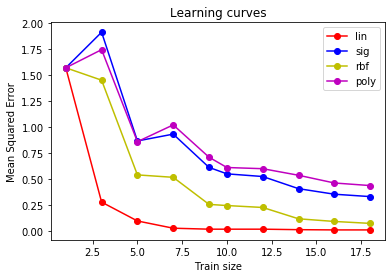
\includegraphics[width=0.7\textwidth]{figures/learncurve.png} %插入图片,[]中设置图片大小,{}中是图片文件名
	\caption{Training results of different SVR kernel functions.} %最终文档中希望显示的图片标题
	\label{fig1} %用于文内引用的标签
	
\end{figure}

As can be seen from figure\ref{fig1}, the results of linear and rbf are much better than the results of sigmoid and polynomial, which all converge to an error close to 0. In fact, the training error of the linear kernel is on the order of $10^{-2}$. Moreover, the linear kernel has already converged by training about ten samples, which shows that our data volume is sufficient for our model.

\subsection{Predicting minimum plastic usage}

From the above analysis, we find that the linear kernel function has the best fitting effect, indicating that the plastic consumption has a linear relationship with the living standard. This is consistent with per capita plastic consumption in different regions. Table \ref{consumption} is a table of plastic consumption in different regions. Intuitively, the consumption of plastic is positively related to the living standard of the region. Developed regions generally have higher plastic consumption. Of course, this is also related to other factors. These are reflected in our model.

\begin{table}[]
	\center
	\caption{Plastic consumption in different regions}
	\begin{tabular}{|c|c|}
		\hline
		\textbf{Area}              & \textbf{\begin{tabular}[c]{@{}c@{}}Plastic consumption\\ (1 ton per 100,000 people)\end{tabular}} \\ \hline
		China                      & 1316.1                                                                                            \\ \hline
		North America              & 1571.9                                                                                            \\ \hline
		Asia Pacific               & 657.1                                                                                             \\ \hline
		Western Europe             & 2870.6                                                                                            \\ \hline
		India                      & 251.9                                                                                             \\ \hline
		Middle East                & 580.4                                                                                             \\ \hline
		Central and South America  & 308.8                                                                                             \\ \hline
		Central and Eastern Europe & 1468.4                                                                                            \\ \hline
		Africa                     & 99.8                                                                                              \\ \hline
		Japan                      & 812.9                                                                                             
		\label{consumption}
		\\ \hline
	\end{tabular}
\end{table}

Based on this conclusion, we found that reducing the amount of plastic used will inevitably affect people's happiness. Therefore, we need to make a compromise between happiness and environment. This is undoubtedly a very painful thing. Therefore, we need to find a threshold on the tolerance of the regions $\kappa$. $\kappa$ is such a value: in a specific area, if happiness $\Gamma = \hat{f}(X) < \kappa$, it is not worthwhile to reduce consumption. Note that $\hat{f}$ is trained in section \ref{train}. $\kappa$ can be derived from historical data and is closely related to each place.

Unfortunately, many people are unwilling to pay a lot for environmental protection\cite{unf}, as is shown in figure \ref{fig3}. So we carefully set this value to 0.5\% of the existing happiness index.

\begin{figure}[!htb] %H为当前位置,!htb为忽略美学标准,htbp为浮动图形
	\centering %图片居中
	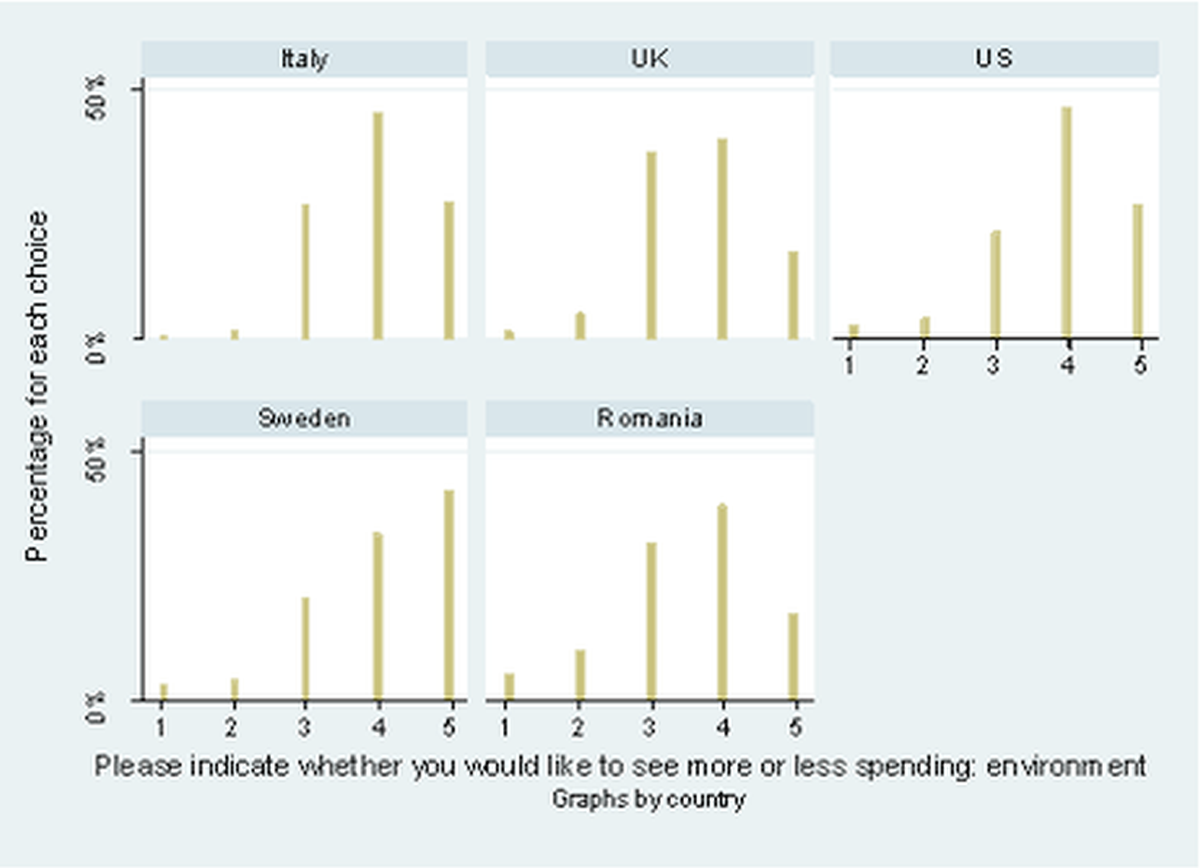
\includegraphics[width=0.7\textwidth]{figures/en.PNG} %插入图片,[]中设置图片大小,{}中是图片文件名
	\caption{Happiness-Plastic curve of US.} %最终文档中希望显示的图片标题
	\label{fig3} %用于文内引用的标签
	
\end{figure}

For example, figure \ref{fig2} shows this relationship in the US. Currently, plastic consumption in the United States is 15.719 kg per people. If the amount of plastic used per person per year in the United States is reduced to 6.19 kg per year, the happiness level in the United States will be reduced by 0.5\%. We think of this as the largest reduction in plastic use in the United States.

%If America's tolerance for happiness is 7.263, then the minimum plastic consumption in the United States should be 500 tons per 100,000 people. If plastics production is required to fall below this limit, it will cause more problems and outweigh the benefits.

\begin{figure}[!htb] %H为当前位置,!htb为忽略美学标准,htbp为浮动图形
	\centering %图片居中
	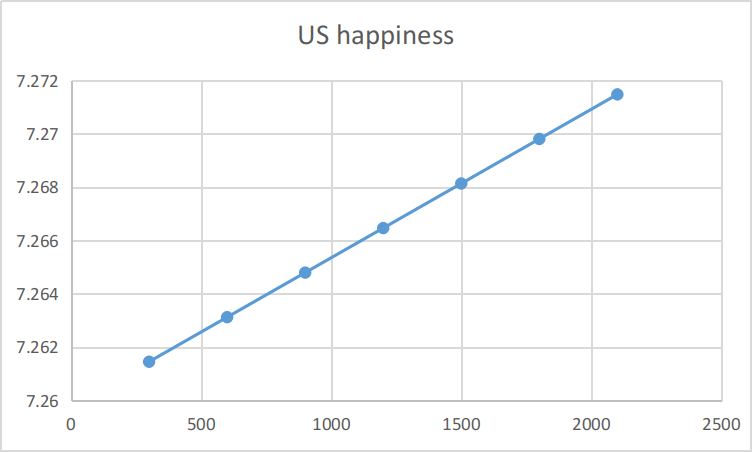
\includegraphics[width=0.7\textwidth]{figures/happiness.png} %插入图片,[]中设置图片大小,{}中是图片文件名
	\caption{Happiness-Plastic curve of US.} %最终文档中希望显示的图片标题
	\label{fig2} %用于文内引用的标签
	
\end{figure}

%We can see from figure \ref{fig2} that using too little plastic can seriously affect people's happiness. Therefore, we can set a threshold to get the smallest amount of plastic that can be used in an area.

%Our solution to this problem is based on the assumption that people will not lead a very difficult life for the reduction of plastic. Based on this, each region has its own minimum tolerable quality of life. By bringing this data into the classifier, we can get the results.

\section{The minimal target of PW and its impacts }

Given that we have get the defined maximal amount of palstic production and the most extent that the plastic waste can be reduced to, taking a statistics of all the regions in the world, we can then get the lowest global target. Next, we analyzed the impact of this measure on human life, environment and plastic industry.

%Given that we have get the defined maximal amount of palstic production and the most extent that the plastic waste can be reduced to, we tend to use dual programing to fine the dual model of PEWM we established first. Then shadow prices of every factor formulated by constraits can be calculated, which indicate the significance of each factor: air, water, carbon dioxide and PW to marine. Then we take several steps to analyze that if the target  is achieved, how the human life, environment and plastic industry will be altered. 

\subsection{Basic Theories}

We have used some theories in this section as a guide, which will be briefly introduced below.

\subsubsection{EASEWASTE}

TheEnvironmental assessment of solid waste systems and technologies (EASEWASTE) is a model that enables waste managers to assess environmental impacts of solid waste management systems and to make comparisons among recovery technologies for a region with a given population and waste generation. Users can define all necessary data for waste composition, collection, treatment, recovery and disposal and life cycle inventory data for materials and energy used in the waste management system\cite{Kirkeby}.

\subsubsection{CGE}

The CGE model explicitly assumes that the behavior of all economic subjects is optimized in accordance with the usual neoclassical microeconomic theory, so it is a model concerned with the behavior of general rather than local economic subjects. It uses the assumption that markets are balanced, not unbalanced, and that all markets are settled at the same time. The basic economic units it analyzes are producers, consumers, governments and foreign economies\cite{CGE}.

\subsubsection{AHP}

AHP has particular application in group decision making and is used around the world in a wide variety of decision situations, in fields such as government, business, industry, healthcare, shipbuilding and education.

Rather than prescribing a "correct" decision, the AHP helps decision makers find one that best suits their goal and their understanding of the problem. It provides a comprehensive and rational framework for structuring a decision problem, for representing and quantifying its elements, for relating those elements to overall goals, and for evaluating alternative solutions\cite{Analytic}.

\subsection{Global Target}

The global goal should be the sum of the small goals in each region. So we divided the world into 10 typical countries according to their plastic assumption amount, as is shown in table \ref{emu}. In a certain category, there are similar plastic assumptions and culture background in a certain category.

For each region, we used the model explained in Section \ref{p2} to calculate the target for minimum plastic use. Global goals can be achieved by adding them together. All details are shown in table \ref{emu}.

\begin{table}[]
	\center
	\caption{Estimated minimum usage for every region.}
	\label{emu}
	\begin{tabular}{|c|c|c|c|}
		\hline
		Region                     & Polulation & Minimum plastic & Estimated minimum usage \\ \hline
		China                      & 13.86      & 425                            & 5890.42                              \\ \hline
		North America              & 3.70       & 619                            & 2290.49                              \\ \hline
		Asia Pacific               & 7.12       & 108                            & 756.01                               \\ \hline
		Western Europe             & 1.41       & 1975                           & 2784.72                              \\ \hline
		India                      & 13.39      & 2700                           & 37087.65                             \\ \hline
		Middle East                & 4.90       & 1875                           & 9188.28                              \\ \hline
		Central and South America  & 6.30       & 1050                           & 6614.18                              \\ \hline
		Central and Eastern Europe & 1.21       & 620                            & 744.01                               \\ \hline
		Africa                     & 12.16      & 49                             & 596.05                               \\ \hline
		Japan                      & 1.28       & 230                            & 291.62                               \\ \hline
	\end{tabular}
\end{table}

Note that the total achievable minimal plastic consumtion obtained is about 6.6 hundred million tons.

\subsection{Impact Path Analysis}

In this section we discuss three most relevant aspects that can be changed: human life, environment and plastic industry.

\subsubsection{How human life will be alert}

In section \ref{p2}, we have discussed how people's happiness index will be affected by the reduction of plastic usage. But happiness only reflect people's satisfaction and quality of life, there are still other possible changes of human life.

For example, living style of most people may be changed. Because the supply of plastic is less than the demand, the price of plastic products is bound to rise. People will be pushed to choose products made of other materials as the succedaneum, which may lead to popularity of new materials in the market. 

But in the long run, less pollution and more substantial development will lead a better quality of life to every one.

\subsubsection{How environment will be affected}

It should be noticed that there is a 2.2 hundred million difference between the maximal and minimal amount of plastics. Since there are part of plastic plastics that should be recycled for realizing the target reduction. Based on LCF thoery, we can use EASEWASTE theory to estimate the positive externalities on the environment of the recovery. The environmental impacts are calculated based on the overall environmental exchanges which comprise resource consumptions and emissions to air, water and soil which in the life cycle impact assessment may contribute to environmental impact potentials\cite{Kirkeby}. 

In section \ref{lp}, we have quantified the negative impacts of plastic production or plastic waste under quite a few assumptions. 
When the plastic waste levels are reduced to target values, the emission harmful gases and carbon dioxide will decline proportionally. The pollution caused by this 2.2 hundred million plastic waste will also be migrated. 

\subsubsection{How to influence plastic industry}

This is one of the few negative effects of this achievement. Some skeptics insist that once limite the production of plastics, the muti- trillion-dollar plastic industry will significantly shrink, which is bad for economic balance especially for countries that developed on primary and secondary industries like China. The accounting loss of a certain country or region could be calculated as:

\begin{equation}
L = O \times P
\end{equation}

where $L$ refers to loss, $O$ is annual output of plastics, and $P$ is annual industory average price of plastics.

Additionally, we should also consider the economic loss or benefit which enrolled the opportunity cost. Computable General Euilibrium(CGE) provide us a fair method to analysis the general influence of this reduction to the plastic industory or even the whole economic. 

CGE suggest that when plastic market come to an equilibrium again after the reduction:

\begin{enumerate}
	\item Producer will switch to other industries and may lead to prosperous of some new and clean materials, which will improve econommic growth and productivity release. 
	\item Consumers will be willing to change their consuming habitats and more likely to accept new products, which will boost domestic demand and stimulate consumption. 
	\item The government can put up new policies to reduce the plastic production by adjusting taxes and import and export quotas, which may adjusts the tax and tarrif policy and make more fiscal revenue. 
\end{enumerate}

\subsubsection{Total impact}

In general, the total impact should be a linear combination of the effects of each factor:

\begin{equation}
I = \sigma _1 i_1 + \sigma_2 i_2 + \sigma_3 i_3 
\end{equation}

where $\sigma_1$, $\sigma_2$ and $\sigma_3$ are the linear coefficients of different factors.

AHP is used to list the matrix and determine the weight of each factor on the whole society. Since the above three factors are abstract social phenomena, we can first quantify the impact with some indicators. Since quantized results have different orders of magnitude and units, we normalize these effects. Multiply the result by the weight of each factor to get the total impact.

Using AHP, we can determine the value of $\sigma_1$, $\sigma_2$ and $\sigma_3$ so that we can calculate the overall impact of different regions. Generally speaking, the weight of different influencing factors in different regions should be different.

\section{Discussion about equity}

The plastic problem is a global problem and requires international cooperation to resolve it. However, the situation is different in different countries or regions, and we cannot generalize. Different countries have different industrial structures and are affected to varying degrees by the reduction in plastic use. Intuitively, the more a country is affected by plastic, the more we should tolerate this country and allow them to reduce the use of plastic at a slower rate. Therefore, in this section, we further analyze the model proposed in section \ref{lp}, and give specific methods to analyze the factors most affected by plastics in a region. Based on this method and continued analysis on Chinese cases, we further give theoretical guidance and relevant suggestions.

\subsection{Shadow price}

We use shadow prices to evaluate the sensitivity of linear programming models. A shadow price is commonly referred to as a monetary value assigned to currently unknowable or difficult-to-calculate costs. It is based on the willingness to pay principle — in the absence of market prices, the most accurate measure of the value of a good or service is what people are willing to give up in order to get it\cite{sp}. Shadow price reflects the value of the optimal use of resources. In the model in Section \ref{lp}, we measured four resources: water quality, air quality, carbon emissions, and marine debris recycling. The shadow prices of these four resources reflect the impact of the region's reduction in plastics on these four resources. 

In our model, resources fall into two categories:

\begin{itemize}
	\item \textbf{Natural resources}. This type of resource is determined by the region itself, and we cannot change the total amount of this resource in a certain region, such as air and water. If the shadow price of this type of resource is high, then we have no choice but to tolerate this area, because forcing such areas to reduce the production and use of plastic will inevitably cause a great burden on the local area.
	\item \textbf{Controllable resources}. This is a resource that can be determined by the actions of a country, such as carbon emissions and the amount of marine debris recovered. If the shadow price of this type of resource is high, we must ask the country or region because it is the inaction of this country that has caused the pollution of plastic waste.
\end{itemize}

For plastic production in a country or region, empirical conclusions often look like this: Developed countries often have better management of plastics and should pay more attention to the issue of natural resources. Developing countries need a lot of resources for development and they should be required to strengthen their management of plastics.

However, this conclusion is not widely applicable, and there are always exceptions. Therefore, for a specific region, the best way is to calculate the shadow price of each resource, so as to truly determine the impact of each resource.

%Therefore, as long as we can obtain the shadow price, we can well solve the problem of unfairness in international cooperation.

%If the shadow price of a certain resource in a region is very large, and this region is in short supply, it is generally not fair to let the region make changes in this resource.

\subsection{Determining shadow prices using dual theory of linear programming}

Two dual linear programming problems can be described like this\cite{Hillier}:

\begin{equation}
\max z = CX
\end{equation}

subject to:

\begin{equation}
\label{d1}
\left\{
\begin{aligned}
AX \le b\\
X \ge 0
\end{aligned}
\right.
\end{equation}

and

\begin{equation}
\max \omega = b^TY
\end{equation}

subject to:

\begin{equation}
\label{d2}
\left\{
\begin{aligned}
A^TY \ge C^T\\
Y \ge 0
\end{aligned}
\right.
\end{equation}

where $C = (c_1,c_2,\cdots,c_n)$, $X = {(x_1,x_2,\cdots,x_n)}^T$, $y = {(y_1,y_2,\cdots,y_m)}^T$, $A$ is a matrix with m rows and n columns, $b = {(b_1,b_2,\cdots,b_m)}^T$.

The shadow price of resources is the dual solution of the linear programming problem $Y^*$ for the following properties:

\begin{itemize}
	\item \textbf{Weak duality.} For any feasible solution of the original problem $X$ and any feasible solution of the dual problem $Y$, there are $CX \le b^TY$.
	\item \textbf{Complementary relaxation.} If $y_i^*>0$, then $\sum_{j=1}{n}a_{ij}x_j^*=b_i$; If $\sum_{j=1}{n}a_{ij}x_j^*<b_i$, then $y_i^*>0$.
\end{itemize}

Based on this conclusion, we can get the following inference: while obtaining the maximum value of the objective function, the Lagrange multiplier\cite{Lagrange} corresponding to each constraint is the shadow price of the resource corresponding to this constraint. Therefore, we only need the Lagrange multiplier for the optimal solution to obtain the shadow price.

\subsection{Shadow price of China's plastic constraint equation: an example}

In this section, we further analyze the constraint equation of plastic consumption in China Eq.\ref{sc} and Eq.\ref{cc}. Based on this, we give the best way for international cooperation for China.

We use MATLAB to obtain the Lagrange multiplier of Eq.\ref{sc} and Eq.\ref{cc} when the optimal solution is obtained, as shown in table \ref{spc}.

\begin{table}[]
	\center
	\caption{Shadow prices of Chinese resources}
	\label{spc}
	\begin{tabular}{|c|c|}
		\hline
		Limiting factor          & Shadow price \\ \hline
		Air                      & $1.63233961552303\times10^{-14}$            \\ \hline
		Water                    & $1.12005836576517\times10^{-17}$            \\ \hline
		Carbon emission          & $5.66607374733818\times10^{-16}$            \\ \hline
		Marine garbage recycling & $2.43902439024392$            \\ \hline
	\end{tabular}
\end{table}

As can be seen from the table \ref{spc}, the shadow price of China's marine garbage recycling volume is much higher than the shadow prices of other influencing factors. This means that the amount of plastic that China can use is actually largely constrained by the amount of marine debris recovered. Part of China's plastic has entered the ocean, but not a lot of it has been recycled. This is an urgent problem. In fact, our model shows that once the constraint is removed, the amount of plastic that can be used normally in China will be much larger than the existing more than one hundred piles, reaching tens of millions of tons. Such a reduction is actually an acceptable burden for China as is analysed in section \ref{p2}.

In terms of natural resources, air has the largest shadow price. For China, priority should be given to reducing the production and use of plastics with more air pollution as much as possible, which will have the most obvious ecological benefits to the region.

\section{Strength and weakness}

%In this section, we will discuss some other details about the model.

The strengths and Weaknesses of our model are summarized as follows:

\subsection{Strengths}

\textbf{Model complexity.} Our model incorporates relevant research results and considers many details, making the model complicated enough to include enough factors. Therefore, our model can analyze the situation in specific regions and draw targeted conclusions, which is conducive to practical use.

\textbf{Agreement between experimental data and real data.} In the process of estimating maximal plastic waste, our model based on PLC theory carefully consider the environmental impact of plastic in different phases of its life cycle rather than merely in the phase of management. What's more, despite the lack of data, our machine learning model still fits the data well. The results of tests on real data sets also validate the performance of our model, where experimental data and real data agrees well. 

\textbf{The amount of data.} In the process of modeling, we extensively collected relevant industry data, making the model sufficiently universal and extensible. To our knowledge, few studies on the relationship between plastics and the environment have been able to model using so much data.

\subsection{Weaknesses}

\textbf{Data accuracy of the model.} In order to consider as many factors as possible, our model introduces more parameters. This makes it difficult to obtain our data, especially when related research is very scarce. Further we will try to simplify the model for different scenarios and improve the usability of the model.

\textbf{Macro analysis.} Our model is too detail-oriented and has insufficient performance in macro analysis. In global research, our model encountered some difficulties and showed some uncertainty. In the future, we will try to explore the relationship between the overall situation and the details, and strive to let our model to show the superiority in global problems, too.

\section{Conclusion}

To mitigate the plastic waste problem, we establish a linear programming base model to estimate the environmental impacts of plastic waste, and get the maximal plastic waste amount without further damage to environment. It is proved that the most extent plastic can be reduced to could be confirmed by HSVR model. A minimal target amount of plastic usage is achieved by expending HSVR model. The equity issue can also be solved by dual programming and sensitivity analysis of factors. Finally, we reckon a timeline to approach this realistic minimal target of plastic using amount. 

\newpage

\begin{thebibliography}{99}
\bibitem{Geyer} Geyer, Roland, Jenna R. Jambeck, and Kara Lavender Law. "Production, use, and fate of all plastics ever made." Science advances 3.7 (2017): e1700782.
\bibitem{Giacovelli} Giacovelli, Claudia. "Single-Use Plastics: A Roadmap for Sustainability." (2018).
\bibitem{LI}LI, Wai Chin, H. F. Tse, and Lincoln Fok. "Plastic waste in the marine environment: A review of sources, occurrence and effects." Science of the Total Environment 566 (2016): 333-349.
\bibitem{Rigamonti}Rigamonti, Lucia, et al. "Environmental evaluation of plastic waste management scenarios." Resources, Conservation and Recycling 85 (2014): 42-53.
\bibitem{Kirkeby}Kirkeby, Janus T., et al. "Environmental assessment of solid waste systems and technologies: EASEWASTE." Waste Management \& Research 24.1 (2006): 3-15.
\bibitem{Smola}Smola, Alex J., and Bernhard Schölkopf. "A tutorial on support vector regression." Statistics and computing 14.3 (2004): 199-222.
\bibitem{World}World Happiness Report. https://kaggle.com/unsdsn/world-happiness. Accessed 15 Feb. 2020.
\bibitem{Plastic}“Plastic Industry Worldwide.” Statista, https://0-www-statista-com.lib.rivier.edu/study/51465/global-plastics-industry/. Accessed 15 Feb. 2020.
\bibitem{SVRs}1.4. Support Vector Machines — Scikit-Learn 0.22.1 Documentation. https://scikit-learn.org/stable/modules/svm.html. Accessed 15 Feb. 2020.
\bibitem{lack}Groot, Jim, et al. "A comprehensive waste collection cost model applied to post-consumer plastic packaging waste." Resources, Conservation and Recycling 85 (2014): 79-87.
\bibitem{book}Andrady, Anthony L., ed. Plastics and the Environment. John Wiley \& Sons, 2003.
\bibitem{kf}“Cross-Validation (Statistics).” Wikipedia, 7 Feb. 2020. Wikipedia, https://en.wikipedia.org/w/index.php?title=Cross-validation\_(statistics)\&oldid=939673086.
\bibitem{McLachlan}McLachlan, Geoffrey J., Kim-Anh Do, and Christophe Ambroise. Analyzing microarray gene expression data. Vol. 422. John Wiley \& Sons, 2005.
\bibitem{unf}Arpad, Todor. “Willing to Pay to Save the Planet? Evaluating Support for Increased Spending on Sustainable Development and Environmentally Friendly Policies in Five Countries.” PLOS ONE, vol. 13, no. 11, Nov. 2018, p. e0207862. PLoS Journals, doi:10.1371/journal.pone.0207862.
\bibitem{Shonfield}Shonfield, Peter. "LCA of management options for mixed waste plastics." WRAP, UK (2008).
\bibitem{Country}Country data. http://data.stats.gov.cn/. Accessed 17 Feb. 2020.
\bibitem{sp}“Shadow Price.” Wikipedia, 11 Dec. 2019. Wikipedia, https://en.wikipedia.org/w/index.php?title=Shadow\_price\&oldid=930271832.
\bibitem{Hillier}Hillier, Frederick S. Introduction to operations research. Tata McGraw-Hill Education, 2012.
\bibitem{Lagrange}“Lagrange Multiplier.” Wikipedia, 17 Dec. 2019. Wikipedia, https://en.wikipedia.org/w/index.php?title=Lagrange\_multiplier\&oldid=931158065.
\bibitem{CGE}CGE model-encyclopedia of MBA think tanks. https://wiki.mbalib.com/wiki/CGE. Accessed 18 Feb. 2020.
\bibitem{Analytic}Analytic Hierarchy Process - Wikipedia. https://en.wikipedia.org/wiki/Analytic\_hierarchy\_process. Accessed 18 Feb. 2020.


\end{thebibliography}


\end{document}
%%
%% This work consists of these files mcmthesis.dtx,
%%                                   figures/ and
%%                                   code/,
%% and the derived files             mcmthesis.cls,
%%                                   mcmthesis-demo.tex,
%%                                   README,
%%                                   LICENSE,
%%                                   mcmthesis.pdf and
%%                                   mcmthesis-demo.pdf.
%%
%% End of file `mcmthesis-demo.tex'.
